%%%%%%%%%%%%%%%%%%%%%%%%%%%%%%%%%%%%%%%%%%%%%%%%%%%%%%%%%%%%%%%%%%%%%%%%%%%%%%%%
%%%%%%%%%%%%%%%%%%   Vorlage für eine Abschlussarbeit   %%%%%%%%%%%%%%%%%%%%%%%%
%%%%%%%%%%%%%%%%%%%%%%%%%%%%%%%%%%%%%%%%%%%%%%%%%%%%%%%%%%%%%%%%%%%%%%%%%%%%%%%%

% Erstellt von Maximilian Nöthe, <maximilian.noethe@tu-dortmund.de>
% ausgelegt für lualatex und Biblatex mit biber

% Kompilieren mit
% lualatex dateiname.tex
% biber dateiname.bcf
% lualatex dateiname.tex
% lualatex dateiname.tex
% oder einfach mit:
% make

\documentclass[
  tucolor,
  BCOR=12mm,     % 12mm binding corrections, adjust to fit your binding
  parskip=half,  % new paragraphs start with half line vertical space
  open=any,      % chapters start on both odd and even pages
  cleardoublepage=plain,  % no header/footer on blank pages
]{tudothesis}


% Warning, if another latex run is needed
\usepackage[aux]{rerunfilecheck}

% just list chapters and sections in the toc, not subsections or smaller
\setcounter{tocdepth}{1}

%------------------------------------------------------------------------------
%------------------------------ Sprache und Schrift: --------------------------
%------------------------------------------------------------------------------
\usepackage{fontspec}
\defaultfontfeatures{Ligatures=TeX}  % -- becomes en-dash etc.

% german language
\usepackage{polyglossia}
\setdefaultlanguage{german}

% for english abstract and english titles in the toc
\setotherlanguages{english}

% intelligent quotation marks, language and nesting sensitive
\usepackage[autostyle]{csquotes}

% microtypographical features, makes the text look nicer on the small scale
\usepackage{microtype}

%------------------------------------------------------------------------------
%------------------------ Für die Matheumgebung--------------------------------
%------------------------------------------------------------------------------

\usepackage{amsmath}
\usepackage{amssymb}
\usepackage{mathtools}

% Enable Unicode-Math and follow the ISO-Standards for typesetting math
\usepackage[
  math-style=ISO,
  bold-style=ISO,
  sans-style=italic,
  nabla=upright,
  partial=upright,
]{unicode-math}
\setmathfont{Latin Modern Math}

% nice, small fracs for the text with \sfrac{}{}
\usepackage{xfrac}


%------------------------------------------------------------------------------
%---------------------------- Numbers and Units -------------------------------
%------------------------------------------------------------------------------

\usepackage[
  locale=DE,
  separate-uncertainty=true,
  per-mode=symbol-or-fraction,
]{siunitx}
\sisetup{math-micro=\text{µ},text-micro=µ}

%------------------------------------------------------------------------------
%-------------------------------- tables  -------------------------------------
%------------------------------------------------------------------------------

\usepackage{booktabs}       % stellt \toprule, \midrule, \bottomrule

%------------------------------------------------------------------------------
%-------------------------------- graphics -------------------------------------
%------------------------------------------------------------------------------

\usepackage{graphicx}
\usepackage{grffile}

% allow figures to be placed in the running text by default:
\usepackage{scrhack}
\usepackage{float}
\floatplacement{figure}{htbp}
\floatplacement{table}{htbp}

% keep figures and tables in the section
\usepackage[section, below]{placeins}


%------------------------------------------------------------------------------
%---------------------- customize list environments ---------------------------
%------------------------------------------------------------------------------

\usepackage{enumitem}

%------------------------------------------------------------------------------
%------------------------------ Bibliographie ---------------------------------
%------------------------------------------------------------------------------

\usepackage[
  backend=biber,   % use modern biber backend
  autolang=hyphen, % load hyphenation rules for if language of bibentry is not
                   % german, has to be loaded with \setotherlanguages
                   % in the references.bib use langid={en} for english sources
]{biblatex}
\addbibresource{references.bib}  % die Bibliographie einbinden
\DefineBibliographyStrings{german}{andothers = {{et\,al\adddot}}}

%------------------------------------------------------------------------------
%------------------------------ Sonstiges: ------------------------------------
%------------------------------------------------------------------------------


\usepackage{braket}%braket schreibweise ermöglichen

\usepackage[pdfusetitle,unicode,linkbordercolor=tugreen]{hyperref}
\usepackage{bookmark}
\usepackage[shortcuts]{extdash}

%------------------------------------------------------------------------------
%-------------------------    Angaben zur Arbeit   ----------------------------
%------------------------------------------------------------------------------

\author{Dag-Björn Hering}
\title{Floquet Theorie für den inversen Faraday Effekt}
\date{2017}
\birthplace{Castrop-Rauxel}
\chair{Lehrstuhl für Theoretische Physik I}
\division{Fakultät Physik}
\thesisclass{Bachelor of Science}
\submissiondate{31. September 2015}
\firstcorrector{Prof.~Dr.~Erstgutachter}
\secondcorrector{Prof.~Dr.~Zweitgutachter}

% tu logo on top of the titlepage
\titlehead{
\includegraphics[height=1.5cm]{logos/tu-logo.pdf}}

\begin{document}
\frontmatter
% \input{content/hints.tex}
\maketitle

% Gutachterseite
\makecorrectorpage

% hier beginnt der Vorspann, nummeriert in römischen Zahlen
\thispagestyle{plain}

\section*{Kurzfassung}
Hier steht eine Kurzfassung der Arbeit in deutscher Sprache inklusive der Zusammenfassung der
Ergebnisse.
Zusammen mit der englischen Zusammenfassung muss sie auf diese Seite passen.

\section*{Abstract}
\begin{english}
The abstract is a short summary of the thesis in English, together with the German summary it has to fit on this page.
\end{english}

\tableofcontents

\mainmatter
% Hier beginnt der Inhalt mit Seite 1 in arabischen Ziffern
\chapter{Einleitung}
In dieser Arbeit wird versucht,
den inversen Faraday Effekt
in einem Bandisolator mit
Hilfe der Floquet Theorie
zu beschreiben.

Der Inverse Farady Effekt (IFE) stellt eine Möglichkeit bereit,
die Magnetisierung in einem Material
durch Bestrahlung zu beeinflussen,
somit bietet er eine interessante
Methode für die
Kontrolle von Magnetisierungsprozessen
 in Nanostrukturen.
Durch ihn werden beispielsweise, wie schon
in Experimenten gezeigt \cite{jackl},
Spin-Wellen in einem Material erzeugt.
Weiterhin bietet er interessante
Aspekte für die Informationstechnik \cite{hertel}).
Als Grundlage für die
theoretische Beschreibung des IFE dient hier
der Artikel "Theory of the inverse Faraday effect
in metals" \cite{hertel} von Riccardo
Hertel, der sich mit dem IFE in Metallen
beschäftigt.

Die Floquet Theorie liefert eine Methode
zur nährungsweisen Berschreibung
getriebener quantenmechanischer Systeme.
Ein Vorteil dieser Theorie ist
die Berücksichtigung der Periodizität
der Störung auf jedem Nährungsschritt.
Ebenfalls ist das Fehlen von
säkularen Termen, die linear oder nicht
periodisch in der Zeit sind, von Vorteil
im Floquet Formalismus.\cite{haenggi}
Sie wird zum Beispiel in dem Artikel \cite{mentink}
dazu genutzt, die Austauschwechselwirkung
in Mott Isolatoren zu untersuchen.
Das Kapitel
"Driven Quantum Systems"
von Peter Hänggi aus dem Buch \cite{haenggi}
dient als Basis für die hier verwendete Floquet Theorie.


In dem Kapitel \ref{sec:theo} werden die
hier benötigten theoretischen Grundlagen
sowohl für den IFE als auch für die Floquet Theorie aufgeführt.
Anschließend wird in Kapitel \ref{sec:model} ein
Modell eines Bandisolators aufgestellt,
in dem der IFE untersucht wird.
Die durch das Modell gewonnenen Ergebnisse
werden in dem Kapitel \ref{sec:ergebnisse} dargelegt.
Abschließend werden in Kapitel \ref{sec:zusamm}
noch einmal die Vorgehensweise
und die gewonnenen Erkenntisse der vorherigen
Kapitel \ref{sec:model} und \ref{sec:ergebnisse}
zusammmengefasst und ein Ausblick
auf noch offene Aspekte gegeben.

%Im Rahmen dieser Bachelorarbeit wird sich mit der Thematik des Inversen Faraday Effektes (IFE) beschäftigt.
%Der IFE bietet eine Möglichkeit zur Kontrolle von ulta schnellen magnetisierungs Prozessen in Nanostrukturen

%sowie die kontrolle von Spinwellen in Materialien   blablabla ist.
%Welcher mit Hilfe der Floquet-Theorie untersucht werden soll.





% hier sollten Verweise auf die Paper stehen wieso inverser Farady effekt interessant
%und  wieso das Floquet theorem von Nutzen ist.

%
%
% \section{Inverser Faraday Effekt}
% Der Inverse Faraday Effekt beschreibt die Enstehung eines Kreisstromes in Materie, welcher
% eine Magnetisierung in dem Material hervorruft, bei Bestrahung mit zirkularpolariesiertem Licht.
%
% Der Inverse Faraday Effekt beschreibt die Enstehung einer Magnetisierung in Materie, die mit zirkularpolariesiertem Licht bestrahlt wird.
% Dabei wird davon ausgegangen, dass die Wechselwirkung primär zwischen dem E-felder der Welle und den Elektronen statt findet.
% Es kann durch mehrere Überlegungen gezeigt werden, dass der Strom, der durch das zirkularpolarisierte Licht erzeugt wird, eine quadratische Abhängigkeit
% zu der E-feld Amplitude besitzt.

\chapter{Theoretische Grundlagen}
\label{sec:theo}
Dieses Kapitel beschäftigt sich mit den
theoretischen Grundlagen, die für diese Arbeit benötigt
werden. Zunächst werden
quantenmechanische Postulate genannt,
die hier Verwendung finden.
Darauffolgend wird eine Methode dargelegt,
den IFE in Metallen
zu beschreiben. Schließlich wird versucht,
die gewonnenen Erkenntnisse über den
IFE in Metallen auf Isolatoren zu übertragen.
Es wird eine Einführung in
die Floquet Theorie gegeben, mit der es möglich
ist, periodische quantenmechanische Systeme
zu beschreiben. Abschließend
wird eine numerische Methode vorgestellt,
um die in der Floquet Theorie beschriebenen
Größen zu berechnen.
In den folgenden Gleichungen werden
\begin{align}
   \symup{e}=\hbar=\text{m}_\symup{e}=\frac{1}{4\pi\epsilon_0}=1
\end{align}
gesetzt.




\section{Postulate der Quantenmechanik}
In der Quantenmechanik wird
ein Zustand eines Systems durch seine Wellenfunktion $\ket{\Psi}$
beschrieben. Die zeitliche Entwicklung solch
eines quantenmechanischen Systems ist durch die
zeitabhängige Schrödingergleichung
\begin{align}
\mathrm{i} \frac{\partial}{\partial t}\ket{{\Psi(t)}}=  H(t) \ket{\Psi(t)} \label{eqn:schrodinger}
\end{align}
mit dem Hamiltonoperator $H(t)$
gegeben.
Für ein zeitunabhängigen Hamiltonoperator wird durch
Separation der Variablen
\begin{align}
  \ket{\Psi(t)}=f(t)\ket{\Psi}
\end{align}
die stationäre Schrödingergleichung
\begin{align}
H \ket{\Psi}_n=E_n\ket{\Psi}_n \label{eqn:stationSG}
\end{align}
mit den Eigenenergien $E_n$ und dem
Eigenzuständen $\ket{\Psi}_n$
hergeleitet.
% Für den zeitabhängigen Teil
% \begin{align}
% \symup{i}\frac{\partial}{\partial t}f(t)=Ef(t)
% \end{align}
% er ... mach ich später
Die Wahrscheinlichkeit $P(t)$ für eine
Wellenfunktion $\ket{\Psi(t)}$
in einem
Zustand $\ket{\phi}$ ist
durch
\begin{align}
  P(t)=\lvert\braket{\phi\vert\Psi}\rvert^2
\end{align}
gegeben.
Observablen des Systems werden durch hermitesche
Operatoren dargestellt.
Der Erwartungswert $\braket{O}$ solch einer Observablen zu
dem Operator $O$
ist durch
\begin{align}
\braket{O}=\braket{\Psi\lvert O\rvert\Psi}
\end{align}
definiert.
\cite{schwabl}


\section{Inverser Faraday Effekt}
\label{sec:inverfaraday}
Der IFE beschreibt die Entstehung eines Kreisstromes
in Materie durch Bestrahlung mit zirkular
 polarisiertem Licht.
Die dabei entstehende Magnetisierung
in der Materie bleibt gegebenenfalls
auch nach Bestrahlung permanent erhalten.
Hier wird zunächst eine Herleitung des
IFE in Metallen
dargelegt und im Anschluss versucht,
die Ergebnisse auf einen Isolator
zu übertragen.
Es wird davon ausgegangen, dass
die Wechselwirkung primär zwischen dem
oszillierenden elektrischen Feld der Welle
\begin{align}
  E(x,t)=\hat{E}\exp{\left(\symup{i}kr-\symup{i}\omega t\right)}
\end{align}
und den Elektronen stattfindet.
Des Weiteren werden ein wechselwirkungsfreies Elektronenplasma angenommen und quantenmechanische Effekte vernachlässigt.
Für die Bestimmung der Stromdichte $j$,
die durch zirkular polarisiertes Licht mit der Frequenz $\omega$ und
der Amplitude $\hat{E}$ des elektrischen Feldes entsteht, dient die Kontinuitätsgleichung
\begin{align}
  \frac{\partial}{\partial t}n +\nabla(nv) \label{eqn:konti}
\end{align}
mit der Elektronendichte $n$ und der Geschwindigkeit $v$
als Ausgangspunkt.
Wobei die Geschwindigkeit $v$ über den Zusammenhang
\begin{align}
  j=env=\sigma E
\end{align}
mit der Stromdichte $j$, dem elektrischen Feld $E$ und
der Leitfähigkeit des bestrahlten Materials $\sigma$
verknüpft ist.
Eine Größe $a$ lässt sich unter Betrachtung von zwei unterschiedlichen Zeitskalen darstellen als
\begin{align}
  a=\braket{a}+\delta a
\end{align}
mit $\braket{a}$ dem zeitlichen Mittelwert der Größe und
$\delta a$ dem oszillierenden Anteil in Zeiteinheiten des elektrischen Feldes.
Durch Anwenden dieser Annahme auf die Größen der
Kontinuitätsgleichung \eqref{eqn:konti}
wird ein Ausdruck für die entstehende Magnetisierung $M$
\begin{align}
  \vec{M}=-\frac{\symup{i}}{4 \braket{n}\omega }\left(\sigma^*\hat{E}^* \times \sigma\hat{E}\right)\label{eqn:magnet}
\end{align}
hergeleitet.
Aus dem Zusammenhang
\begin{align}
\braket{j}=\nabla\times M \label{eqn:nabla}
\end{align}
ergibt sich die mittlere Stromdichte $\braket{j}$,
die für die Magnetisierung $M$ verantwortlich ist.
Für den Fall einer links bzw. rechts zirkular polarisierten Welle
mit der Ausbreitungsrichtung in $\vec{e}_z$ gilt
\begin{align}
  \hat E \times \hat{E}^*=\pm\symup{i}\lvert E\rvert^2\cdot \vec{e}_z.
\end{align}
Durch Einsetzen der Leitfähigkeit
für ein wechselwirkungsfreies Elektronenplasma
\begin{align}
\sigma=\frac{\symup{i}\braket{n}}{\omega}
\end{align}
in die Gleichung \eqref{eqn:magnet}
ergibt sich die Magnetisierung in einem Metall,
welches mit rechts bzw. links zirkular polarisiertem
Licht in $\vec{e}_z$-Richtung
bestrahlt wird, zu
\begin{align}
  M=\pm\frac{\symup{i}\braket{n}}{4\omega^3}\lvert\hat{E}\rvert^2 \vec{e}_z.
\end{align}
Es ist eine Antiproportionalität
zur dritten Potenz in $\omega$
und eine quadratische Abhängigkeit in $\hat{E}$
für die Magnetisierung und somit auch für den Strommittelwert
zu erkennen. \cite{hertel}

Um eine Voraussage zu den Abhängigkeiten, die
bei dem IFE in einem Bandisolator auftreten,
zu treffen, wird die Leitfähigkeit
eines Isolators
\begin{align}
  \sigma=\symup{i}\omega C
\end{align}
mit der materialabhängigen Konstante $C$
ebenfalls in die Gleichung \eqref{eqn:magnet}
eingesetzt.\cite{fließebach}
Für die Magnetisierung in einem Bandisolator, der mit
rechts bzw. links zirkular polarisiertem Licht bestrahlt wird,
ergibt sich
\begin{align}
  \vec{M}=\pm\frac{\omega C^2}{4\braket{n}} \lvert \hat{E}  \rvert^2 \vec{e}_z. \label{eqn:iso}
\end{align}
Die Gleichung \eqref{eqn:iso}
sagt somit für den IFE in Isolatoren
eine Magnetisierung
vorher, die
linear
in der Frequenz $\omega$ und
quadratisch in dem Betrag der Amplitude des elektrischen
Feldes $\lvert\hat{E}\vert$ ist.
% Dies gilt ebenfalls
% für den zeitlichen
% Strommittelwert, welcher sich aus
% der Gleichung \eqref{eqn:nabla} ergibt.



\newpage
\section{Floquet Theorie}
\label{sec:floquetheo}
In diesem Abschnitt werden die Grundlagen der
Floquet Theorie vorgestellt. Diese wird
dazu genutzt,
um ein in der Zeit periodisches quantenmechanisches System zu beschreiben.
Die zeitliche Entwicklung für so ein System
ist durch die zeitabhängige
Schrödingergleichung  \eqref{eqn:schrodinger}
gegeben. Wobei der Hamiltonian die Bedingungen
\begin{align}
  &H(t)=H(t+T),
\intertext{und}
  H(t)&=H_0+V(t)  &\text{mit}&   &V(t)=V(t+T)
\end{align}
erfüllen muss.
ER ist also periodisch
in der Zeit
und kann als Summe von einem
ungestörten Anteil $H_0$
und einem in der Zeit periodischen
Potential $V(t)$ geschrieben werden.
Das Floquet Theorem besagt, dass Zustände
 $\ket{\Psi_{\alpha}(t)}$ existieren,
welche Lösungen
von \eqref{eqn:schrodinger} sind, die
die Form
\begin{align}
\ket{\Psi(t)_\alpha}=\exp\left(-\mathrm{i}\epsilon_\alpha\right)\ket{\Phi_\alpha(t)}\label{eqn:psi_a}
\intertext{haben. Dabei ist $\ket{\Phi_\alpha(t)}$ eine sogenannte Floquet Mode und
unterliegt der periodischen Bedingung}
\ket{\Phi_\alpha(t)}=\ket{\Phi_\alpha(t+T)}.
\end{align}
Der Parameter $\epsilon_\alpha$ ist real und
wird auch charakteristischer Exponent oder
Floquet Exponent genannt.
Mit Hilfe von \eqref{eqn:psi_a} lässt sich
die Schrödingergleichung \eqref{eqn:schrodinger}
in die Form
\begin{align}
\mathcal{H}(t)\ket{\Phi_\alpha(t)}=\epsilon_\alpha \ket{\Phi_\alpha(t)} \label{eqn:floquetgl.}
\intertext{bringen, wobei der Operator }
  \mathcal{H}(t)=\left( H(t)-\mathrm{i}\frac{\partial}{\partial t} \right)
\end{align}
ist. Durch die Ähnlichkeit der Gleichung
\eqref{eqn:floquetgl.} zu der stationären
Schrödingergleichung
werden $\epsilon_\alpha$ und $\phi_\alpha$
auch als Quasieigenenergien und Quasieigenzustände,
im Folgendem abgekürzt mit QEE und QEZ,
bezeichnet.
Darüber hinaus ist
\begin{align}
  \ket{\Phi_{\alpha '}(t)}=\ket{\Phi_\alpha(t)}\exp(\mathrm{i}n\omega t) \equiv \ket{\Phi_{\alpha n}(t)}
\end{align}
ebenfalls eine Lösung von \eqref{eqn:floquetgl.},
wobei $n \in \mathbb{Z} / \{0 \} $
und $\omega$ die Frequenz des Potentials ist.
Dies hat eine Änderung der QEE in der Form
\begin{align}
    \epsilon_\alpha \rightarrow \epsilon_{\alpha '}=\epsilon_\alpha+n\omega\equiv\epsilon_{\alpha n} \label{eqn:epsilon_n}
\end{align}
zufolge.
Durch diese Feststellung ist es
möglich, alle QEE
für unterschiedliche $\alpha$
in der ersten Brillouin-Zone darzustellen,
da sich alle weiteren
QEE über \eqref{eqn:epsilon_n}
berechnen lassen.
Die QEZ unterliegen der Orthogonaliätsbedingung
\begin{align}
  \braket{\braket{\Phi_{\alpha' }(t)|\Phi_{\beta'}(t)}}\equiv \frac{1}{T} \int_0^T\mathrm{d}t
  \braket{\Phi_{\alpha' }(t)|\Phi_{\beta'}(t)}=\delta_{\alpha'\beta'}=\delta_{\alpha\beta}\delta_{nm}. \label{eqn:ortho}
\end{align}
Um die zeitliche Entwicklung
eines Startzustandes $\ket{\Psi(0)}$
mit der Floquet Theorie durchzuführen,
wird
zunächst der Startzustand $\ket{\Psi(0)}$ durch
die Superposition der QEZ
\begin{align}
  \ket{\Psi(0)}=\sum_\alpha c_a\ket{\Phi_\alpha(0)}& &\text{mit}&  &c_\alpha=\braket{\Phi_\alpha|\Psi(0)} \label{eqn:super}
\end{align}
ausgedrückt.
Der Zeitpropagator der Floquet Theorie
\begin{align}
  K(t;0)=\sum_\alpha \exp\left(-\mathrm{i}\epsilon_\alpha t \right)\ket{\Phi_\alpha(t)}\bra{\Phi_\alpha(0)} \label{eqn:Propagator}
\end{align}
ermöglicht,
den Startzustand \eqref{eqn:super}
in der Zeit zu propagieren.
Die Anwendung dieses Propagators auf den Startzustand
\eqref{eqn:super}
liefert
\begin{align}
  \ket{\Psi(t)}=K(t;0) \ket{\Psi(0)}=\sum_\alpha c_\alpha \exp\left(-\mathrm{i}\epsilon_\alpha t \right)\ket{\Phi_\alpha(t)}. \label{eqn:psi_t}
\end{align}
\cite{haenggi},\cite{dr}
% !!!!! in die Ergebnisse !!!!! Mit Hilfe dieses Propagators ist es unkomplizit in dem Floquet Formalismus, zeitlichgemittelte (read) Erwartungswerte von
% Operatoren $\hat O$ zu berechnen.
% Das zeitliche Mittel ist gegeben durch
% \begin{align}
%   \bar{\hat O}= \frac{1}{T}\int_0^T \braket{\Psi(t)|O|\Psi(t)}
% \intertext{Durch Einsetzen von \eqref{eqn:psi_t} und \eqref{eqn:fourier} ergibt sich nach Ausführung der Integration}
%  \bar{\hat O}= \sum_\alpha \lvert c_\alpha \rvert^2  \sum_{-\infty}^{\infty} c_\alpha^n(x)^\dag \hat{O} c_\alpha^n (x)^{\phantom{\dag}}.
% \end{align}
%
% Eine Herleitung dieser Formel ist im Anhang zu finden.??
\newpage
\section{Floquet Matrix Methode}
\label{sec:matrix}
Im Folgenden wird die numerische Methode
der Floquet Matrix,
welche die Berechnung der QEE
$\epsilon_{\alpha}$ und QEZ
$\ket{\Phi_\alpha}$  ermöglicht, vorgestellt.
Die QEZ $\Phi_\alpha$ lassen sich, da es
sich um in der Zeit periodische Zustände handelt,
als Fourierreihe
\begin{align}
  \ket{\Phi_{\alpha}(t)}&=\lim_{N\to\infty}\sum_{n=-N}^{N} \exp(\mathrm{i}n\omega t) \ket{c_{\alpha}^n} \label{eqn:fourier}
 \intertext{mit}
 \ket{c_\alpha^n}&=\sum_{k=1}^D c_{\alpha,k}^n \ket{\varphi_k} %phi beliebiges orthonomal set auf h_0
\end{align}
darstellen.
Hierbei ist $\ket{\varphi_k}$ ein beliebiges
orthonormales Set auf $H_0$ mit der Dimension $D$.
Durch Einsetzen von \eqref{eqn:fourier} in \eqref{eqn:floquetgl.}
ergibt sich die Definition der Matrixelemente
\begin{align}
  \braket{\bra{\varphi_j m}\mathcal{H}_\mathrm{F}\ket{\varphi_k n}}\equiv \braket{\varphi_j|H^{m-n}|\varphi_k} + n \omega \delta_{n,m}\delta_{j,k} \label{eqn:H_f}
\intertext{mit}
H^{m-n}=\frac{1}{T}\int_0^T \mathrm{d}t H(t) \exp\left(-\mathrm{i}(m-n)\omega t\right) \label{eqn:H_n_m}
\end{align}
mittels denen sich die Floquet Matrix $\mathcal{H}_\mathrm{F}$ aufstellen lässt.
Aus der Lösung der Eigenwertgleichung
\begin{align}
  \mathrm{det}|\mathcal{H}_\mathrm{F}-\epsilon\mathbb{1}|=0
\end{align}
folgen die QEE $\epsilon_{\alpha,n}$ und die Eigenvektoren $\ket{\epsilon_{\alpha,n}}$.
Diese QEE
genügen den periodischen Bedingungen aus der Gleichung \eqref{eqn:epsilon_n}.
Um aus den Eigenvektoren $\ket{\epsilon_{\alpha,n}}$
die QEZ  $\ket{\Phi_{\alpha}(t)}$
zu bestimmen, wird die Gleichung \ref{eqn:fourier}
verwendet.
Die vektorartigen Entwicklungskoeffizienten $\ket{c_\alpha^n}$ können den
Eigenvektoren der QEE, die sich in der 1. Brillouin-Zone
befinden, entnommen werden.
Dabei entsprechen die Komponenten
der Eigenvektoren, welche zu der
$n$-ten Fourier Mode gehören,
den Komponeten $c_{\alpha,k}^n$.
\cite{haenggi},\cite{dr}

\chapter{Modellierung des IFE in einem Bandisolator}
\label{sec:model}
%\section{Hameltonien}
Um den IFE mit Hilfe der Floquet Theorie in
einem Bandisolator genauer zu untersuchen, wird hier ein
mikroskopisches zwei dimensionales Modell
eines Festkörpers mit vier Gitterplätzen herangezogen. Zu Beginn
wird ein System betrachtet, in dem sich ein spinloses
Elektron aufhält, wobei zwischen dem
zeitunabhängigen System ohne ein elektrisches Feld
und dem zeitabhängigen System mit einem in der Zeit
periodischen elektrischen Feld unterschieden wird.
Darauffolgend wird die Floquet Matrix nach dem Abschnitt
\ref{sec:matrix} für das
zeitabhängige System aufgestellt. Abschließend wird das
System für zwei spinlose Elektronen betrachtet.


\section{Zeitunabhängiges System}
Dieses Gittersystem wird durch das
Tight-Binding-Modell in zweiter Quantisierung
mit periodischen Randbedingungen \cite{czycholl} beschrieben.
Aus diesem ergibt sich der folgende Hamiltonian $H_0$
für das zeitunabhängige System % lautet
\begin{align}
  H_0=\underbrace{J\sum_{i=1}^4 \left(c_{i+1}^\dag c_i^{\phantom{\dag}} + c_{i}^\dag c_{i+1}^{\phantom{\dag}}\right)}_{H_{TB}}
   +\underbrace{\sum_{i=1}^4\left( a_i^{\phantom{\dag}} c_i^\dag c_i^{\phantom{\dag}} \right)}_{H_a},
\end{align}
wobei der Tight-Binding Hamiltonian $H_{TB}$, der die Sprünge des Elektrons
zwischen den Gitterplätzen beschreibt, mit dem Hamiltonian $H_a$, der die Eigenschaften
eines Bandisolators simuliert, erweitert wird.
Dabei besitzen die Gitterplätze eine lokale alternierende Energie $a$.
Die Gitterplätze sind im Abstand der Gitterkonstanten $d$ quadratisch angeordnet.
In der Abbildung \ref{fig:system}
ist eine Skizze des zu untersuchenden Systems dargestellt.
\begin{figure}
   \centering
   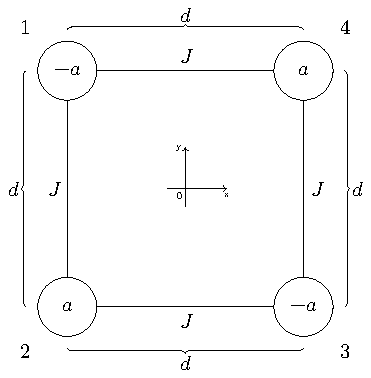
\includegraphics[width=0.4\textwidth]{Programme/Tikz_test/bild_gitter_0.pdf}
   \caption{Skizze des verwendeten 2D-Modells
    des Bandisolators mit vier Gitterplätzen im Abstand $d$,
   welche die alternierende lokale Energie $a$ besitzen.
    Elektronen im System können abhängig von dem Tight-Binding-Paramter $J$
   den Gitterplatz wechseln.}
   \label{fig:system}
\end{figure}
Durch die Wahl der Basis
\begin{align}
\ket{1}=\vec{e}_{1}&  \ket{2}=\vec{e}_2&   &\ket{3}=\vec{e}_3& &\ket{4}=\vec{e}_4,&
\intertext{mit den Einheitsvektoren $\vec{e}_i$ wird über}
H_{ij}&=\braket{i|H|j}
\end{align}
eine Matrixdarstellung des Hamiltonians
\begin{align}
  H_0&=\begin{pmatrix}
  -a          & \phantom{-}J &\phantom{-}0& \phantom{-}J \\
  \phantom{-}J& \phantom{-}a &\phantom{-}J& \phantom{-}0\\
  \phantom{-}0& \phantom{-}J & -a         & \phantom{-}J \\
  \phantom{-}J& \phantom{-}0&\phantom{-}J & \phantom{-}a
\end{pmatrix}
\end{align}
bestimmt.
Mit Hilfe der stationären Schrödingergleichung \ref{eqn:stat}
ergeben sich die Eigenwerte
\begin{align}
  E_{1/4}&=\mp\sqrt{a^2+4J^2}&  &E_{2/3}=\mp a
\end{align}
und die Eigenvektoren $\ket{\phi}_n$  des Hamiltonians.
Die Eigenwerte $E_n$ des Hamiltonians
sind in der Abbildung \ref{fig:bandstruktur}
in einem Niveauschema dargestellt.
\begin{figure}
   \centering
   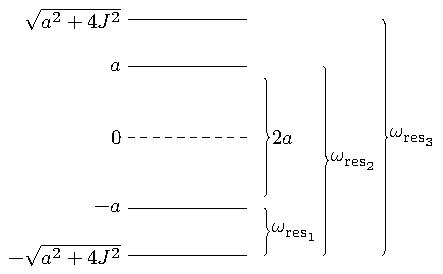
\includegraphics[width=0.4\textwidth]{Programme/Tikz_test/bild_niveau.pdf}
   \caption{Niveauschema für ein Elektron, welches sich in dem System befindet
und die dadurch resultierende Bandlücke $2a$ und
mögliche Resonanzfrequenzen des Systems.}
   \label{fig:bandstruktur}
\end{figure}

%Ebenfalls kann die für ein Bandisolator charakteristische Bandlücke von $2a$
Die möglichen Resonanzfrequenzen des Systems im Grundzustand
\begin{align}
\omega_{\text{res}_1}=\sqrt{a^2+4J^2}-a,
& &\omega_{\text{res}_2}=a+\sqrt{a^2+4J^2},
& &\omega_{\text{res}_3}=2\sqrt{a^2+4J^2} \label{eqn:Resonanz}
\end{align}
werden aus dem Niveauschema \ref{fig:bandstruktur}
entnommen. In der Abbildung
\ref{fig:bandstruktur} ist ebenfalls die Bandlücke $2a$
dargestellt.

\section{Zeitabhängiges System}
Als nächstes wird das System durch ein rotierendes E-Feld erweitert, welches
das zirkular polarisierte Licht simulieren soll,
zu sehen in der Abbildung \ref{fig:syst+E}.

\begin{figure}
   \centering
   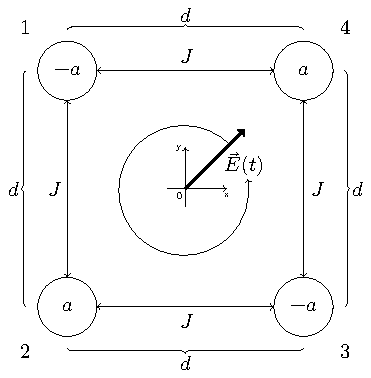
\includegraphics[width=0.4\textwidth]{Programme/Tikz_test/bild_gitter.pdf}
   \caption{Skizze des zeitabhängigen 2D-Modells
bei dem zusätzlich zum zeitunabhängigen Modell
ein mit der Zeit rotierendes elektrisches Feld
eingezeichnet ist.}
 \label{fig:syst+E}
\end{figure}


Der Hamiltonian wird dafür um den Term
\begin{align}
  H_\text{E-Feld}=\sum_{i=1}^4\left(\epsilon_i^{\phantom{\dag}} c_i^\dag c_i^{\phantom{\dag}}\right)& &\text{mit}& &\epsilon&=-\vec{E}(t) \vec{r_i}
\end{align}
erweitert. Dabei beschreibt $H_\text{E-Feld}$ die Welchelwirkung zwischen dem elektrischen Feld
\begin{align}
  \vec E(t)=E_0\begin{pmatrix}
\cos\left(\omega t\right)\\
\sin\left(\omega t\right)
 \end{pmatrix},
\end{align}
welches die Amplitude $E_0$ und
die Frequenz $\omega$ besitzt.
Der Ursprung des Systems wird
in den Mittelpunkt des Systems gesetzt.
Somit lauten die Gitterplatz-Vektoren
$\vec{r_i}$ in Abhänigigkeit von der
Gitterkonstante $d$:
\begin{align}
  \vec{r}_1=\frac{d}{2}\begin{pmatrix}-1  \\ \phantom{-}1 \end{pmatrix},& &
  \vec{r}_2=\frac{d}{2}\begin{pmatrix}-1  \\ -1 \end{pmatrix},& &
  \vec{r}_3=\frac{d}{2}\begin{pmatrix}\phantom{-}1  \\ -1 \end{pmatrix},& &
  \vec{r}_4=\frac{d}{2}\begin{pmatrix}1  \\ 1 \end{pmatrix}.
\end{align}
Der gesamte Hamiltonian des Systems nimmt somit die Form
\begin{align}
%H=J\sum_{i=1}^4 \left(c_{i+1}^\dag c_i^{\phantom{\dag}} + c_{i}^\dag c_{i+1}^{\phantom{\dag}}   +a_i^{\phantom{\dag}} c_i^\dag c_i^{\phantom{\dag}} +\epsilon_i^{\phantom{\dag}} c_i^\dag c_i^{\phantom{\dag}}\right)\\
H=\underbrace{J\sum_{i=1}^4 \left(c_{i+1}^\dag c_i^{\phantom{\dag}} + c_{i}^\dag c_{i+1}^{\phantom{\dag}}\right)}_{H_{TB}}
+\underbrace{\sum_{i=1}^4 \left(a_i^{\phantom{\dag}} c_i^\dag c_i^{\phantom{\dag}}\right)}_{H_a}
+\underbrace{\sum_{i=1}^4 \left(\epsilon^{\phantom{\dag}}_i c_i^\dag c_i^{\phantom{\dag}}\right)}_{H_\text{E-Feld}}
\end{align}
an.


\section{Floquet Matrix des zeitabhängigen Systems}
Für das zeitabhängige System wird wie
in Kapitel \ref{sec:matrix} beschrieben, die
numerische Methode der Floquet Matrix angewendet.
Dafür wird zunächst der Hamiltonian
\begin{align}
H=\underbrace{J\sum_{i=1}^4 \left(c_{i+1}^\dag c_i^{\phantom{\dag}} + c_{i}^\dag c_{i+1}^{\phantom{\dag}}c_i^{\phantom{\dag}}\right)
+ \sum_{i=1}^4\left(a_i^{\phantom{\dag}} c_i^\dag c_i^{\phantom{\dag}}\right)}_{H_0}
-\underbrace{\sum_{i=1}^4\left(\vec{E} \vec{r_i}  c_i^\dag c_i^{\phantom{\dag}}\right)}_{V(t)}
\end{align}
in den zeitunabhängigen Teil $H_0$ und einen in der
 Zeit periodischen Teil $V(t)$ aufgespalten.
Um die Floquet Matrix $\mathcal{H}_\mathrm{F}$ zu berechnen, werden zunächst die Untermatrizen $H^{m-n}$ bestimmt.
Aus der Gleichung \eqref{eqn:H_n_m} folgt
\begin{align}
 H^{m-n}&=H_0\delta_{m,n} -\frac{E_0}{2}\left(R_{(-)} \delta_{n+1,m} + R_{(+)}\delta_{n-1,m}\right)
 \intertext{mit}
  R_{(-)}&=\textbf{diag}\left(
  r_{1_x}-r_{1_y} ;
  r_{2_x}-r_{2_y} ;
  r_{3_x}-r_{3_y} ;
  r_{4_x}-r_{4_y}\right)
\\
  R_{(+)}&= \textbf{diag}\left(
  r_{1_x}+r_{1_y} ;
  r_{2_x}+r_{2_y} ;
  r_{3_x}+r_{3_y} ;
  r_{4_x}+r_{4_y}\right).
\end{align}
Somit ergibt sich die Matrix $\mathcal{H}_F$
nach der Gleichung \eqref{eqn:H_f} in
Blockschreibweise zu einer Diagonalbandmatrix.
% \begin{align}
%   \mathcal{H}_F=\begin{pmatrix}
%   H^{-n ,-n}+(-n)\hbar\omega  &  H^{-n,-n+1}       &       &    & \\
%   H^{-n+1,-n} &    H^{-n+1,-n+1}+(1-n)\hbar\omega  & \ddots&    & \\
%             &          \ddots                      & \ddots&  \ddots      &    \\
%             &                                      & \ddots&  H^{n-1,n-1}+(n-1)\hbar\omega  & H^{n-1,n}  \\
%             &                                      &       & H^{n,n-1}   & H^{n,n}
% \end{pmatrix}
% \end{align}
Für exakte $\epsilon_{\alpha}$ und $\ket{\Phi_\alpha}$ muss
$N\rightarrow\infty$ gehen,
da dies numerisch jedoch nicht möglich ist, wird
die Matrix $\mathcal{H}_F$ bei
einem beliebigen $N$ trunkiert.
Dadurch werden nur die Fouriermoden bis $N$ in der
Berechnung der QEE und QEZ
berücksichtigt.
Die Matrix $\mathcal{H}_F$ besitzt beispielsweise
für einen Trunkierparameter $N=1$ die Form
\begin{align}
  \mathcal{H}_F=\begin{pmatrix}
  H^{-1,-1}-\hbar\omega\mathbb{1} &  H^{-1,0} &   0 \\
  H^{0,-1}               &  H^{0,0}  &H^{0,1}                  \\
      0                  &  H^{1,0}  & H^{1,1}+\hbar\omega\mathbb{1}
\end{pmatrix}.
\end{align}

\section{Zwei-Elektronen-System}
Dem Modell wird ein Elektron
hinzugefügt, in Folge dessen
unterliegt das System dem Pauliverbot.
Die Eigenwerte $E_n$ setzen sich dabei aus
linear Kombinationen der Eigenwerte
des Ein-Elektron-Systems
zusammen \cite{phillip} zu
\begin{align}
E_{1/4}&=\mp\sqrt{a^2+4J^2}-a
&E_{2/6}&=\mp\sqrt{a^2+4J^2}+a
&E_{3/4}&=0.
\end{align}
Somit besitzt das System im Grundzustand die möglichen Resonanzfrequenzen
\begin{align}
\omega_{\text{res}_1}&=2a
&\omega_{\text{res}_{2/3}}&=\sqrt{a^2+4J^2}+a \\
\omega_{\text{res}_4}&=2\sqrt{a^2+4J^2}
&\omega_{\text{res}_5}&=2\sqrt{a^2+4J^2}+2a.
\end{align}
Wird dem Modell wieder ein Elektron
hinzugefügt und es somit auf ein
Drei-Elektronen-System erweitert, ist es
möglich, das Modell als ein System
zu betrachten, welches nur ein
Teilchen mit positiver Ladung enthält.
Diese Betrachtung liefert dasselbe Ergebnis
wie das Ein-Elektron-System und
ist somit trivial. \cite{phillip}

\chapter{Ergebnisse}
\label{sec:ergebnisse}
In diesem Kapitel werden zu Beginn
Eigenschaften der Floquet Theorie an dem Modell überprüft.
Weiterhin wird die zeitliche Entwicklung
eines Zustandes durch den
Floquet Formalismus mit der einer numerischen Lösung der
Schrödingergleichung verglichen.
Auf zwei unterschiedliche Weisen wird jeweils ein in der Zeit
gemittelter Strom berechnet und miteinander verglichen.
IFE abhänigkeiten überprüfen
Anschließend wird das Zwei-Elektronen-System betrachtet und ebenfalls ein gemittelter Strom berechnet.

In den folgenden Rechnungen wird der Sprungterm J auf $1\si{\electronvolt}$ gesetzt und
für den Gitterabstand wird eine typischen Wert von $d=\SI{4}{\angstrom}$ fest gewählt.
Alle anderen Größen werden im Folgenden in Einheiten von $J$ und $d$ angegeben.
Die Bandlücke $2a$ sollte in den Größenordnung des Sprungtermes $J$ liegen und wird
daher auf $2J$ gesetzt.
Die Parameter des elektrischen Feldes werden im Bezug auf das in \cite{jackl} beschriebene Experiment gewählt.
Die Amplitude der Elektrischenfeldes liegt somit um den Wert
\begin{align}
  E_0=\SI{69,2}{\mega\volt\per\meter}=0,028\, \frac{J}{d\symup{e}}.
\end{align}
Eine typische Frequenz des Feldes ist dann
\begin{align}
  \omega\approx\SI{2,35}{\peta\hertz}=1,549\frac{J}{\hbar}.
\end{align}
Des weiteren wird eine Pulsdauer $\mathcal{T}=\SI{50}{\femto\second}\approx75,96\,\frac{\hbar}{J}$
für das Lichtfeld eingeführt, indem das System beobachtet wird.

Eigenwerte und Eigenvektoren einer Matrix werden mit der Funktion \textit{eig} aus dem Programm Octave \cite{octave}
berechnet. Weitere Rechnungen wurden mit Pyhon ...



\section{Frequenzabbhängigkeit der Quasienergien}
Zunächst werden die Eigenschaften der Floquet Theorie,
teils unabhängig von typischen Größen des Systems, untersucht. Dafür
werden die Eigenwerte
 $\epsilon_{\alpha n}$ für eine
Matrix $\mathcal{H}_\mathrm{F}$ mit der
Größe $N=1$,  konstanter lokaler Energie $a=1\,J$
und E-Feldamplitude $E_0=1\,\frac{J}{d\symup{e}}$
für Frequenz in einem Bereich von $0\,\frac{J}{\hbar}-6\,\frac{J}{\hbar}$  berechnet.
Um die Effekte der Störung $V(t)$ zu verdeutlichen,
werden ebenfalls Eigenwerte $E_{\alpha n}$ für Matrix $\mathcal{H}_F$ mit $E_0=0\frac{J}{d\symup{e}}$, dies besschreibt den
zeitunabhänigen Fall, berechnet, sodass in Abbildung \ref{fig:epsilon_f}
die berechneten Eigenwerte verglichen werden können.
\begin{figure}
   \centering
   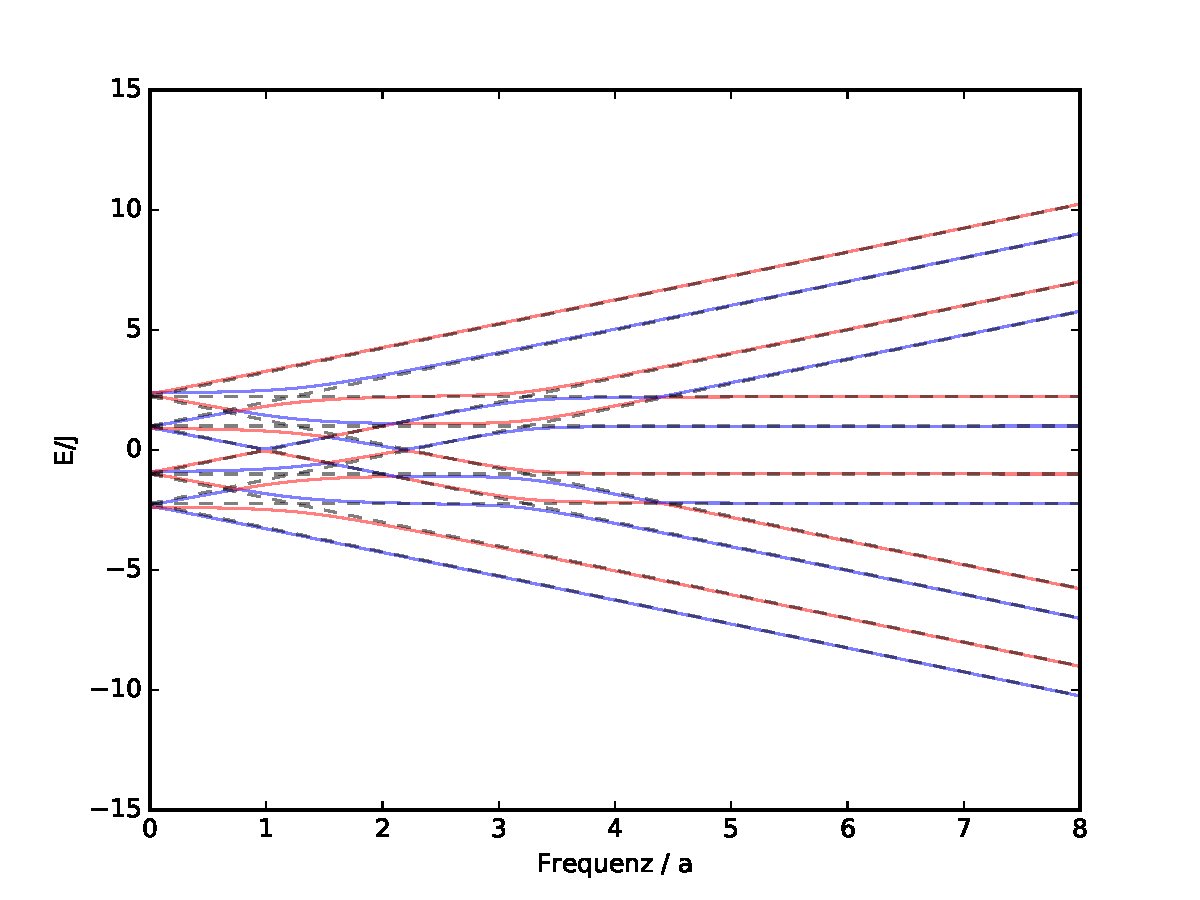
\includegraphics[width=0.7\textwidth]{Programme/Freqenzen_kontinuierlich/Plots/Plot_fur_a=1.0_E=1.0.pdf}
   \caption{Eigenwerte $\epsilon_{\alpha n}$ der Matrix $\mathcal{H}_\mathrm{F}$ für $a=1\,J$ und $E_0=1\,\frac{J}{d\symup{e}}$ und
   Eigenwerte $E_{\alpha n}$ des zeitunabhängigen System in Abhängigkeit von der Frequnez $\omega$.}
   \label{fig:epsilon_f}
\end{figure}
In der Abbildung \ref{fig:epsilon_f} können, wie in \cite{haenggi} beschrieben, an Stellen der Überschneidung der Eigenwerte  $E_{\alpha n}$
des zeitunabhängigen Systems die Phänomene des "avoided crossing" und
"exact crossing" der Quasienergien $\epsilon_{\alpha n}$ beobachtet werden,
die durch das zeitabhängige elektrische Feld hervorgerufen werden.
??vielleicht erklären??
Dies dient hier als Bestätigung der Funktionsweise
des aufgestellten Algorithmus für die Matrix-Methode und wird im Folgendem nicht weiter behandelt.

\section{Brillouin-Zone der Quasienergien}
In diesem Abschitt wird die Darstellung der Quasienergien, wie in
Abschitt \ref{sec:flotheo} beschrieben, in der 1.
Brillouin-Zone untersucht.
Dafür werden Quasienergien bei einer konstanten Frequenz $\omega=1\,\frac{J}{\hbar}$ und
lokalen Energie $a=1\,J$ in Abhängigkeit der
Amplitude $E_0$, die hier unabhängig
von realistischen Werten zur besseren Veranschaulichung im
Bereich $0\,\frac{J}{d\symup{e}}<E_0<5\,\frac{J}{d\symup{e}}$ liegt, berechnet.
Diese sind in der Abbildung \ref{fig:brillouin} gegen $E_0$ aufgetragen.
Zusätzlich wird der Trunkierparameter $N$ der Matrix $\mathcal{H}_F$ variiert.

\begin{figure}
  \centering
  \begin{subfigure}{0.48\textwidth}
    \includegraphics[width=1\textwidth]{Programme/Energien_kontinuierlich/Plots/Plot_fur_a=1.0_w=1.0N=1.0.pdf}
    \caption{N=1}
    \label{fig=N_1}
  \end{subfigure}
  \begin{subfigure}{0.48\textwidth}
    \includegraphics[width=1\textwidth]{Programme/Energien_kontinuierlich/Plots/Plot_fur_a=1.0_w=1.0N=3.0.pdf}
    \caption{N=3}
    \label{fig=N_3}
  \end{subfigure}
  \begin{subfigure}{0.48\textwidth}
    \includegraphics[width=1\textwidth]{Programme/Energien_kontinuierlich/Plots/Plot_fur_a=1.0_w=1.0N=5.0.pdf}
    \caption{N=5}
    \label{fig=N_5}
  \end{subfigure}
  \begin{subfigure}{0.48\textwidth}
    \includegraphics[width=1\textwidth]{Programme/Energien_kontinuierlich/Plots/Plot_fur_a=1.0_w=1.0N=6.0.pdf}
    \caption{N=6}
    \label{fig=N_6}
  \end{subfigure}
  \caption{Berechnete $\epsilon_{\alpha n}$ für unterschiedliche Größen der Matrix $\mathcal{H}_F$
  bei einer lokalen Energie $a=1\,J$ und einer Frequenz $\omega=1\frac{J}{\hbar}$ in der 1. und 2. Brillouin Zone}
  \label{fig:brillouin}
\end{figure}

Deutlich wird, dass für kleine Trunkierparamter $N$ die Bedingung für eine Darstellung in der 1. Brillouin-Zone nicht erfüllt ist.
Es wird jedoch beobachtet, dass die Übereinstimmung der 2. Brillouin-Zonen mit der  1. Brillouin-Zone mit
größeren $N$ zunimmt.
Somit können die Quasienergien $\epsilon_\alpha$  für ein ausreichend großes $N$ in die erste Brillouin-Zone
mit $-\frac{\omega}{2}<\epsilon_\alpha<\frac{\omega}{2}$ dargestellt und
alle anderen Quasienergien $\epsilon_{\alpha n}$ durch die Periodizitätsbedingung \eqref{eqn:epsilon_n} berechnet werden.
In der ersten Brillouin-Zone, siehe Abbildung \ref{fig:brillouin}, existieren genau vier Quasienergien, folglich besitzt das System
ebenfalls vier Quasienergien und vier Quasizustände.
%Aus der  Abbildung \ref{fig:brillouin} kann entnommen werden, System vier Quasienergien besitzt

\section{Orthogonalität der Quasizustände}
Im Folgenden soll die Orthogonalität zwischen den Quasizuständen $\ket{\Phi_\alpha}$ aus der Gleichung \eqref{eqn:ortho} für
unterschiedliche Trunkierparameter $N$ für die Matrix $\mathcal{H}_F$ überprüft werden.
In der Abbildung \ref{fig:ortho} ist das Skalarprodukt zwischen den Quasizuständen in Abhängigkeit von der Größe $N$ der Matrix
$\mathcal{H}_F$
für die Werte    $a=1\, J$ , $E_0=0,028\,\frac{J}{d\symup{e}}$  und $\omega=1\,\frac{J}{\hbar}$ , welche im typischen Bereich liegen,
dargestellt.

\begin{figure}
    \centering     % vielleicht mit 2x2 subfigure
    \includegraphics[width=0.7\textwidth]{Programme/Orthogonalitat_der_quasizustande/Plots/Potential=1.0/Energie=0.028/Frequenz=1.0/Plot_fur_phi1_phi_i}
    \caption{Das Skalarprodukt $\braket{\Phi_1|\Phi_i}$ folgt auch für die anderen Zustände}
     \label{fig:ortho}
\end{figure}

Aus Abbildung \ref{fig:ortho} wird entnommen, dass bei bei geringem parameter $N$ die Orthogonalität der Quasizustände
nicht gegeben ist.
Für die in Abbildung \ref{fig:ortho} verwendeten Größen
erweist sich eine Größe von $N=3$ als ausreichend zur Gewährleistung der Orthogonalität.
Es estellt sich weiterhin ein antiproportionler Zusammenhang von lokaler Energie $a$ und Frequenz $\omega$ zu der
benötigten Größe $N$ der Matrix $\mathcal{H}_F$
heraus.
Wegen der antiproportionalität ist es notwendig,
bei den folgenden Berechnungen für
Werte von $\omega$ und $a$, die kleiner als die in Abbildung
\ref{fig:ortho} gewählten Werte sind, die
Orthogonalität der Quasizustände zu überprüfen.
Andernfalls reicht eine Matrixgröße von $N=3$ zum Erfüllen der Orthogonalitätsbedingung aus.



% -über formel .. kann quasizustand berechnet werden
% -die Orthogonalitäts bedingung formel .. sollte erfüllt sein

\section{Zeitentwicklung eines Zustandes durch den Floquet Formalismus}
In den Abschitten
In diesem Abschnitt wird eine Zeitentwicklung des Ein-Elektron-Systems mit oszillierendem E-Feld durch den Floquet Formalismus bestimmt.
Als Startzustand $\ket{\Psi_0}$ wird der Grundzustand $\ket{\phi_1}$ des zeitunabhänigen Systems verwendet, da
dass das System zu Beginn im Zustand niedrigster Energie verweilt.
Es sollen zunächst werden Frequenzen $\omega$ abseits einer Resonanzfrequenz des E-Feldes
betrachtet.
In der Abbildung \ref{fig:Resonanz} sind
 die Resonanzfrequenzen \eqref{eqn:Resonanz} in Abhängigkeit
von den lokalen Energien aufgetragen.

\begin{figure}
  \centering
  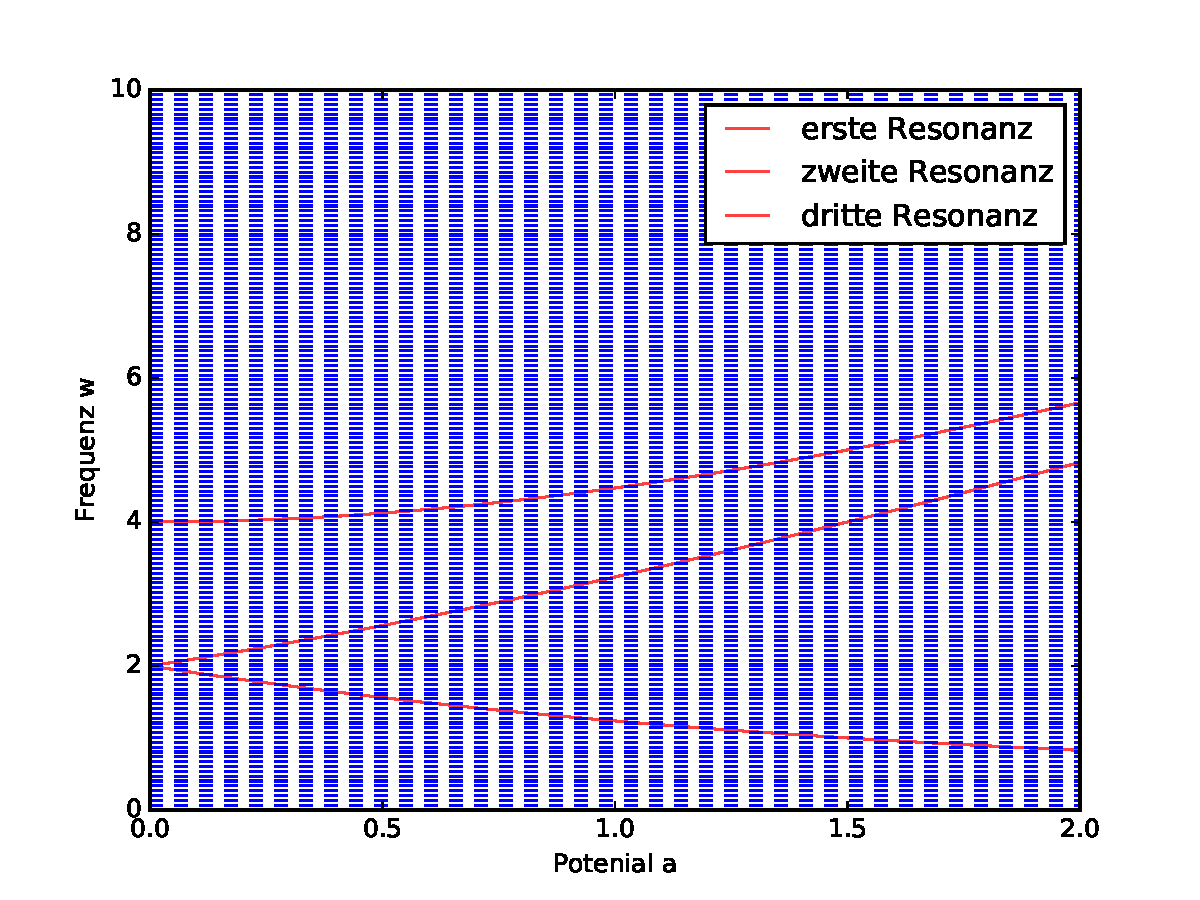
\includegraphics[width=0.7\textwidth]{Programme/Eigenzustande/Plots/Resonanzen.pdf}
  \caption{Resonanzfrequenzen in Abhängigkeit von der lokalen Energie $a$}
  \label{fig:Resonanz}
\end{figure}


Unter dem Ausschluss der Resonanzfrequenzen aus der
Abbildung \ref{fig:Resonanz}, wird bei einer lokalen Energie
$a=0,5$ und einer Amplitude $E_0=0,028\,\frac{J}{d\symup{e}}$ die Frequenz $\omega=1,549\,\frac{J}{\hbar}$ gewählt.
Um die Zeitentwicklung nach Floquet durchführen zu können, muss
zunächst, wie in Gleichung \eqref{eqn:superposition} beschrieben, der Grundzustand
als Superposition der Quasizustände ausgedrückt werden.
Durch Anwenden des Zeitpropagators \eqref{eqn:Propagator} auf den Grundzustand,
 ist es somit möglich den zeitentwickelten Grundzustand
$\ket{\Psi(t)}$ zu berechnen.

In Abbildung \ref{fig:zeitentwicklung} ist
die Aufenthaltswahrscheinlichkeit
$\lvert\braket{e_i|\Psi(t)}\rvert^2$ für
die vier unterschiedlichen Gitterplätze in Abhängigkeit von der Zeit dargestellt.
Dabei wird ebenfalls eine numerische Lösung
der Schrödingergleichung für den Grundzustand durch den
adaptiven Algorithmus $\textit{lsode}$,
der durch das Programm Octave \cite{octave}bereitgestellt wird, aufgetragen.

\begin{figure}
  \centering
  \includegraphics[width=0.7\textwidth]{Programme/Eigenzustande/Plots/Potential=1.0/Energie=0.028/Besetzungen(t)_mit_Floquet_N=3w=1.549.pdf}
  \caption{Zeitenwicklung des Grundzustandes}
  \label{fig:zeitentwicklung}
\end{figure}

Es zeigt sich, dass die verschiedenen Lösungen übereinstimmen. Somit kann die Lösung der Floquet Theorie bestätigt werden.
Auffällig ist, dass die Gitterplätze $1$ und $3$
bevorzugt sind, dies kann durch die Struktur des Bandisolators begründet werden, da
die beiden Position eine geringere lokale Energie $a$ besitzen.
%
% -wenn Zustände orthogonal zeitentwicklung möglich
% -vergleich mit lsode
% -stimmt überein eignet sich folglich für zeitentwicklung

\section{Untersuchung des Stromes im Bandisolators}
In dem vorherigen Abschnitt konnte die Zeitentwicklung der Floquet Theorie betätigt werden.
Diese zuvor Bestätigte zeitentwicklungwird hier zur Berechnung des Stromes in dem System genutzt.
Durch
\begin{align}
\braket{I}(t)=\braket{\psi(t)\lvert I \rvert\psi(t)}
\intertext{mit dem Stromdichteoperator\cite{schwabl}}
I= \frac{\symup{i}J}{4}\sum_i^4 c_{i+1}^\dag c_{i}^{\phantom{\dag}}  -c_{i}^\dag c_{i+1}^{\phantom{\dag}}
\end{align}
ergibt sich der Stromfluss des Systems.
Wird $\ket{e_i}$ wieder als Basis gewählt, ergibt sich
die Matrixdarstellung des Strom(dichte)operators
\begin{align}
I=\frac{\symup{i}J}{4}\begin{pmatrix}
  \phantom{-}0&           -1 &\phantom{-}0 & \phantom{-}1 \\
  \phantom{-}1& \phantom{-}0 &          -1 & \phantom{-}0\\
  \phantom{-}0& \phantom{-}1 &\phantom{-}0 &           -1 \\
            -1& \phantom{-}0 &\phantom{-}1 & \phantom{-}0
\end{pmatrix}.
\end{align}
Die Abbildung \ref{fig:strom_t} enthält den Stromfluss des Systems in Abhängigkeit von der Zeit.

\begin{figure}
  \centering
  \includegraphics[width=0.7\textwidth]{Programme/Strom/Plots/Potential=1.0/Energie=0.028/Stromerwartungswert(t)_N=3w=1.549.pdf}
  \caption{Strom im System in Abhängigkeit der Zeit}
 \label{fig:strom_t}
\end{figure}



Die Messung  des Stromes $\braket{I}(t)$ auf so kleinen Zeitskalen ist jedoch nicht möglich, daher
misst der Beobachter nur einen in der Zeit gemittelten Strom
\begin{align}
  \bar{\braket{I}}= \frac{1}{T}\int_0^T \braket{\Psi(t)|I|\Psi(t)}.
\end{align}
Mit Hilfe des Zeitpropagators \eqref{eqn:prop} ist es in dem Floquet Formalismus problemlos möglich, zeitlich
gemittelte Erwartungswerte von
Operatoren zu berechnen.
Das zeitliche Mittel über eine große Zeitspanne??? eine Periode $T$ ist gegeben durch
\begin{align}
  \bar{\braket{O}}= \frac{1}{T}\int_0^T \braket{\Psi(t)|O|\Psi(t)}.
\intertext{Durch Einsetzen von \eqref{eqn:psi_t} und \eqref{eqn:fourier}
 ergibt sich}
 \bar{\braket{O}}&= \sum_\alpha \lvert c_\alpha \rvert^2  \sum_{-\infty}^{\infty} \braket{c_\alpha^n\lvert O \rvert c_\alpha^n}  \label{eqn:mittel} \text{\cite{gespräch}}
 \intertext{mit}
  c_\alpha&=\braket{\Psi_0\vert\Phi_\alpha}
\end{align}
nach Ausführung der Integration.
??In dem Floquet Formalismus ist es somit nicht notwendig die Erwartungswerte
 zu berechnen und diese über eine
Zeitspanne zu mitteln. Durch die Formel \eqref{eqn:mittel} kann
der gemittelte Erwartungswert unkompliziert berechnet werden.??
Zur Überprüfung der Gleichung \eqref{eqn:mittel} wird
der gemittelte Stromerwartungswert $\bar{\braket{I}}$
für unterschiedliche Frequenzen $\omega$
in Abhängigkeit von der Amplitude des elektrischen Feldes $E_0$
zum einen durch die Gleichung \ref{eqn:mittel}
und zum anderen über die Mittelung über eine
lange Zeitspanne, hier
T=??,  ??mehrere Perioden?? des berechneten
Erwartungswert des Stromes $\braket{I}(t)$ bestimmt.
Die Abbildung \ref{fig:E_Strom} enthält jeweils die aus
den zwei verschiedenen Methoden für $a=1$
berechneten gemittelten Ströme $\bar{\braket{I}}$.


\begin{figure}
  \centering
  \includegraphics[width=0.7\textwidth]{Programme/Strom_mittelwerte/Plots_mittelwerte/Potential=1.0Stromerwartungswert(t)_N=3.pdf}
  \caption{mittelwert des Stromerwartungswert für die zweite Methode wurde über die Pulsdauer $\mathcal{T}$ Zeit Spanne von ?? gemittelt }
  \label{fig:E_Strom}
\end{figure}


Aus der Abbildung \ref{fig:E_strom} kann entnommen werden,
dass die Gleichung \ref{eqn:mittel} identische
Ergebnisse wie die zweite Methode liefert.
Somit ist bestätigt, dass der zeitlichgeittel
Stromerwartungswert $\bar{\braket{I}}$
über die Gleichung \ref{eqn:mittel}
berechnet werden kann.
Im Folgenden wird ??(nur) die Methode,
die die Floquet Theorie bereitstellt,
um zeitlich gemittelte Stromerwartungswerte zu berechnen,
verwendet.

\section{Überprüfung der Strom Abhängigkeiten in einem Bandisolators}
Wie in dem Kapitel \ref{sec:inverfaraday} beschrieben,
soll der Strom bei dem IFE??(Inverser Faraday Effekt)
in einem Isolator quadratisch
mit der Amplitude des elektrischen Feldes $E_0$
sowie linear mit der Frequenz $\omega$ des elektrischen
Feldes steigen. Diese Abhängikeiten sollen nun für den
 Ein-Elektronen-Fall überprüft werden.
Für die quadratische Abhängigkeit wird in der Abbildung
\ref{fig:E_abb} der zeitliche Strommittelwert $\bar{\braket{I}}$
 gegen $E_0$ aufgetragen.
Genutzt werden
vier Frequenzen, die jeweils zwischen den Resonanzen liegen, um Resonanzeffekte zu vermeiden.
Es wird eine lokale Energie von $a=0,5$ und Frequenzen von $\omega=1,2,3,5$,
die jeweils die Bedingung erfüllen, verwendet.
An die berechneten Werte wird versucht eine quadratische Funktion $f(x)=ax^2$
anzulegen\footnote{Mit Hilfe von python \textit{curvefit} }, ebenfalls zu sehen
in Abbildung \ref{fig:E_abb}.

\begin{figure}
  \centering
  \includegraphics[width=0.7\textwidth]{Programme/Strom_fit_e/Plots_mittelwerte/Potential=1.0Stromerwartungswert(t)_N=3.pdf}
  \caption{Überprüfung der $E_0$ abhängigkeiten.}
  \label{fig:E_abb}
\end{figure}

Es ist möglich, eine quadratische Funktion anzulegen,
folglich kann die quadratische Abbhängigkeit
bestätigt werden.

Abschließend gilt es, die Linearität des Strommittelwertes
 zu der Frequenz zu untersuchen.
Hierfür wird der Strommittelwert $\bar{\braket{I}}$
in Abhängigkeit von der Frequenz $\omega$ in einem
Bereich von $0$ bis $8$ für
zwei verschiedene elektrische Amplituden $E_0=??,??$
untersucht, siehe Abbildung \ref{fig:I_freq}.
Erneut wird eine lokale Energie von $a=0,5$???? variieren ???? verwendet.

\begin{figure}
   \centering
   \includegraphics[width=0.7\textwidth]{Programme/Strom_frequenzabb/Plots_mittelwerte/Potential=1.0Stromerwartungswert(t)_N=3.pdf}
   \caption{Strom in Abhängigkeit von der Frequenz}
   \label{fig:w_abb}
\end{figure}


In der Abbildung können Resonanzeffekte
bei den zuvor berechneten Resonanzfrequenzen
beobachtet werden. Auf Grund der
dominierenden Resonanzeffekte in Abbildung \ref{fig:w_abb}
lässt sich die Linearität nicht eindeutig bestätigen.
Um die Resonanzeffekte zu ??vernächlässigen??, soll ein kleinerer Frequenzbereich, hier von
$0-0,8$, untersucht werden.
Jedoch fällt der Strom in diesem Bereich ??'unnormal'??
ab. Als Ursache hierfür kann eine in diesem
Frequenzbereich nicht mehr gewährleistete Orthogonalität der
Quasizustände sein, da zuvor nur eine minimale Frequenz
von $\omega=1$ auf Orthogonalität überprüft wurde.
Um dies zu untersuchen, wird das Skalarprodukt der Quasizustände gegen
die Frequenz \omega in der Abbildung \ref{fig:N_5} für $N=5$ aufgetragen.
%Dies geschieht ebenfalls für  $N=10$, $N=20$ und $N=50$

\begin{figure}
   \centering
   \begin{subfigure}{0.48\textwidth}
       \includegraphics[width=1\textwidth]{Programme/Orthogonalitat_der_quasizustande_frequenz/Plots/Potential=1.0/Energie=0.028/Anzahl=3/Plot_fur_phi1_phi_i.pdf}
       \caption{N=3}
       \label{fig:N_3}
     \end{subfigure}
     \begin{subfigure}{0.48\textwidth}
       \includegraphics[width=1\textwidth]{Programme/Orthogonalitat_der_quasizustande_frequenz/Plots/Potential=1.0/Energie=0.028/Anzahl=10/Plot_fur_phi1_phi_i.pdf}
       \caption{N=50}
       \label{fig:N_10}
     \end{subfigure}
     \begin{subfigure}{0.48\textwidth}
       \includegraphics[width=1\textwidth]{Programme/Orthogonalitat_der_quasizustande_frequenz/Plots/Potential=1.0/Energie=0.028/Anzahl=20/Plot_fur_phi1_phi_i.pdf}
       \caption{N=50}
       \label{fig:N_20}
     \end{subfigure}
     \begin{subfigure}{0.48\textwidth}
       \includegraphics[width=1\textwidth]{Programme/Orthogonalitat_der_quasizustande_frequenz/Plots/Potential=1.0/Energie=0.028/Anzahl=50/Plot_fur_phi1_phi_i.pdf}
       \caption{N=50}
       \label{fig:N_50}
     \end{subfigure}
        \caption{Das Skalarprodukt }
    \label{fig:N_gross}
\end{figure}


Die Abbildung \ref{fig:N_5} bestätigt
die Vermutung der fehlenden Orthogonalität.
Folglich muss die Größe $N$ der Matrix
$\mathcal{H}_F$ erhöht werden.
Die Abbildung \ref{fig:N_gross} enthält ebenfalls
den gleichen Zusammenhang
aus \ref{fig:N_5} jedoch für
größere $N$.
Es zeigt sich, dass für höhere $N$ geringere Frequenz
erreicht werden können, welche die orthogonalität Bedingung
erfüllen. Allerdings
ist der Zusammenhang ?'noch nicht klar'?(Antiproportional).
Als Konsequenz folgt, dass für geringere
Frequenzen die Matrix zu groß wird und nicht
mehr unkompliziert diagonalisierbar ist.
Demzufolge ist es notwendig, bei Untersuchung des linearen Bereiches eine
größere Matrix $\mathcal{H}_F$ aufzustellen. Hier soll $N=50$ genügen,
folglich dürfen Frequenzen kleiner als $0,1??$ bei der Überprüfung der Linearität nicht
berücksichtigt werden.
Der Strommittelwert $\bar{\braket{\mathcal{J}}}$
 wird im zuvor geforderten Frequenzbereich $0-0,8$
gegen $\omega$ aufgetragen, siehe Abbildung \ref{fig:geraden_fit}.
Bei Frequenzen um $0,7??$
machen sich bereits Resonanzeffekte bemerkbar,
deshalb wird versucht eine Gerade im Frequenzbereich $0,1??$-$0,5??$
an die berechneten Werte anzupassen. ??Fitten??.

\begin{figure}
    \centering
    \includegraphics[width=0.7\textwidth]{Programme/Strom_geraden_fit/Plots_mittelwerte/Potential=1.0Stromerwartungswert(t)_N=50.pdf}
    \caption{Geraden fit}
    \label{fig:geraden_fit}
\end{figure}

Die berechneten Werte und die Gerade liegen übereinander.
Aufgrund dessen kann der lineare Zusammenhang in diesem Frequenzbereich bestätigt werden.

% -berechung des Stromes
% -überprüfung der quadratischen Ahängigkeit der Stromes
% -frequenz abhängigkeit überprüfen (gerade)
% -für kleine frequenz problem mit orthogonalität

\section{Zwei-Elektronen-System}
Um einen Strommittelwert $\bar{\braket{\symup{J}}}$
in dem Zwei-Elektronen-System,
welches sich im Grunzustand befindet, zu berechnen,
wird der Strommittelwert $\bar{\braket{\symup{J}}}$
für ein Ein-Elektronen-System
sowohl im Grundzustand als
auch im ersten Angeregeten Zustand
berechnet. Aus Addition der beiden
Ein-Elektron-Ströme ergibt sich der Strom
des Zwei-Elektronen-System.
Die Abbildung \ref{fig:2e} enthält
den Strommittelwert des Zwei-Elektronen-Systems
in Abhänigkeit der Amplitude
des Elektrischen Feldes $E_0$.
Wieder wird das System
unterschiedliche Frequenz $\omega=??$
beobachtet.

% \begin{figure}
%     \centering
%     \includegraphics[width=0.7\textwidth]{Programme/Strom_geraden_fit/Plots_mittelwerte/Potential=0.5Stromerwartungswert(t)_N=50.pdf}
%     \caption{Zwei-Elektronen-System}
%     \label{fig:2e}
% \end{figure}

\chapter{Zusammenfassung und Ausblick}


\appendix
% Hier beginnt der Anhang, nummeriert in lateinischen Buchstaben
\chapter{Ein Anhangskapitel}

Hier könnte ein Anhang stehen, falls Sie z.B. Code, Konstruktionszeichnungen oder Ähnliches mit in die Arbeit bringen wollen. Im Normalfall stehen jedoch alle Ihre Resultate im Hauptteil der Bachelorarbeit und ein Anhang ist überflüssig.


\backmatter
\printbibliography

\cleardoublepage
\thispagestyle{empty}
\section*{Eidesstattliche Versicherung}
Ich versichere hiermit an Eides statt, dass ich die vorliegende Abschlussarbeit mit dem Titel \enquote{\thetitle} selbstständig und ohne unzulässige fremde Hilfe erbracht habe.
Ich habe keine anderen als die angegebenen Quellen und Hilfsmittel benutzt, sowie wörtliche und sinngemäße Zitate kenntlich gemacht. 
Die Arbeit hat in gleicher oder ähnlicher Form noch keiner Prüfungsbehörde vorgelegen.

\vspace*{1cm}\noindent
\begin{center}
  \begin{tabular}{@{}p{0.4\textwidth}@{\hspace{0.15\textwidth}}p{0.4\textwidth}@{}}
  \rule{\linewidth}{0.25pt}& \rule{\linewidth}{0.25pt}\\
  Ort, Datum & Unterschrift
  \end{tabular}
\end{center}

\subsection*{Belehrung}
Wer vorsätzlich gegen eine die Täuschung über Prüfungsleistungen betreffende Regelung einer Hochschulprüfungsordnung verstößt, handelt ordnungswidrig.
Die Ordnungswidrigkeit kann mit einer Geldbuße von bis zu \SI[round-mode=places, round-precision=2]{50000}{€} geahndet werden. 
Zuständige Verwaltungsbehörde für die Verfolgung und Ahndung von Ordnungswidrigkeiten ist der Kanzler/die Kanzlerin der Technischen Universität Dortmund. 
Im Falle eines mehrfachen oder sonstigen schwerwiegenden Täuschungsversuches kann der Prüfling zudem exmatrikuliert werden \mbox{(\S\,63 Abs. 5 Hochschulgesetz --HG--).}

Die Abgabe einer falschen Versicherung an Eides statt wird mit Freiheitsstrafe bis zu 3 Jahren oder mit Geldstrafe bestraft.

Die Technische Universität Dortmund wird ggf.\ elektronische Vergleichswerkzeuge (wie z.\,B.\ die Software \enquote{turnitin}) zur Überprüfung von Ordnungswidrigkeiten in Prüfungsverfahren nutzen. \\[\baselineskip]

\noindent Die oben stehende Belehrung habe ich zur Kenntnis genommen.\\[1cm]
\begin{center}
\begin{tabular}{@{}p{0.4\textwidth}@{\hspace{0.15\textwidth}}p{0.4\textwidth}@{}}
\rule{\linewidth}{0.25pt}& \rule{\linewidth}{0.25pt}\\
Ort, Datum & Unterschrift
\end{tabular}
\end{center}

\end{document}
